\pdfminorversion=4
\documentclass[aspectratio=169]{beamer}

\mode<presentation>
{
  \usetheme{default}
  \usecolortheme{default}
  \usefonttheme{default}
  \setbeamertemplate{navigation symbols}{}
  \setbeamertemplate{caption}[numbered]
  \setbeamertemplate{footline}[frame number]  % or "page number"
  \setbeamercolor{frametitle}{fg=white}
  \setbeamercolor{footline}{fg=black}
} 

\usepackage[english]{babel}
\usepackage{inputenc}
\usepackage{tikz}
\usepackage{courier}
\usepackage{array}
\usepackage{bold-extra}
\usepackage{minted}
\usepackage[thicklines]{cancel}
\usepackage{fancyvrb}

\xdefinecolor{dianablue}{rgb}{0.18,0.24,0.31}
\xdefinecolor{darkblue}{rgb}{0.1,0.1,0.7}
\xdefinecolor{darkgreen}{rgb}{0,0.5,0}
\xdefinecolor{darkgrey}{rgb}{0.35,0.35,0.35}
\xdefinecolor{darkorange}{rgb}{0.8,0.5,0}
\xdefinecolor{darkred}{rgb}{0.7,0,0}
\definecolor{darkgreen}{rgb}{0,0.6,0}
\definecolor{mauve}{rgb}{0.58,0,0.82}

\title[2024-08-19-python-school-setting-stage]{Fast and Efficient Python Programmming School: \\ Setting the Scene}
\author{Jim Pivarski}
\institute{Princeton University -- IRIS-HEP}
\date{August 19, 2024}

\usetikzlibrary{shapes.callouts}

%% Thanks to https://github.com/gpoore/minted/issues/288
\makeatletter
%
% Similar to \EscVerb.
%
% \EscMintinline[options]{<language>}{<backslash-escaped text>}
%
\def\EscMintinline{%
  \FVExtraRobustCommand
  \RobustEscMintinline
  \FVExtraUnexpandedReadOArgMArgEscVArg}

\NewExpandableDocumentCommand \FVExtraUnexpandedReadOArgMArgEscVArg { o m m } {%
  \IfNoValueTF{#1}
    {\FVExtraAlwaysUnexpanded
      {\FVExtraUnexpandedReadOArgMArgEscVArg{#2}{#3}}}
    {\FVExtraAlwaysUnexpanded
      {\FVExtraUnexpandedReadOArgMArgEscVArg[#1]{#2}{#3}}}%
}

\newrobustcmd\RobustEscMintinline[2][]{%
  % similar to \mintinline
  \begingroup
  \setboolean{minted@isinline}{true}%
  \minted@configlang{#2}%
  \setkeys{minted@opt@cmd}{#1}%
  \minted@fvset
  \begingroup
  \@ifnextchar\bgroup
    {\FVExtraDetokenizeREscVArg{\minted@inline@iii}}%
    {\PackageError{minted}%
     {\string\EscMintinline\space delimiters must be paired curly braces in this context}%
     {Delimit argument with curly braces}}}
\makeatother

\begin{document}

\logo{\pgfputat{\pgfxy(0.11, 7.4)}{\pgfbox[right,base]{\tikz{\filldraw[fill=dianablue, draw=none] (0 cm, 0 cm) rectangle (50 cm, 1 cm);}\mbox{\hspace{-8 cm}
\includegraphics[height=1 cm]{princeton-logo-long.png}\hspace{0.1 cm}\raisebox{0.1 cm}{
\includegraphics[height=0.8 cm]{iris-hep-logo-long.png}}\hspace{0.1 cm}}}}}

\begin{frame}
  \titlepage
\end{frame}

\logo{\pgfputat{\pgfxy(0.11, 7.4)}{\pgfbox[right,base]{\tikz{\filldraw[fill=dianablue, draw=none] (0 cm, 0 cm) rectangle (50 cm, 1 cm);}\mbox{\hspace{-8 cm}
\includegraphics[height=1 cm]{princeton-logo.png}\hspace{0.1 cm}\raisebox{0.1 cm}{
\includegraphics[height=0.8 cm]{iris-hep-logo.png}}\hspace{0.1 cm}}}}}

% Uncomment these lines for an automatically generated outline.
%\begin{frame}{Outline}
%  \tableofcontents
%\end{frame}

% START START START START START START START START START START START START START

\begin{frame}{Welcome!}
\vspace{0.5 cm}

\includegraphics[width=\linewidth]{img/aachen-school-banner.png}
\end{frame}

\begin{frame}{Setting the scene: Python and performance}
\vspace{0.3 cm}
\begin{center}
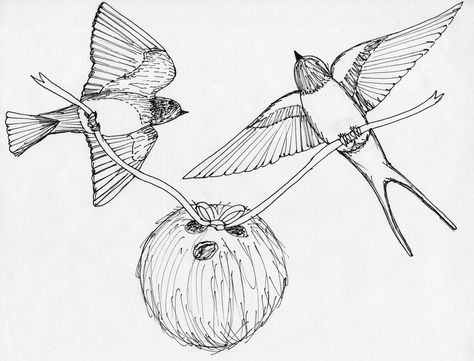
\includegraphics[width=0.7\linewidth]{img/swallows-coconut.jpg}
\end{center}
\end{frame}

\begin{frame}{Big, oversimplified history}
\vspace{-1.3 cm}
\begin{center}
\only<1>{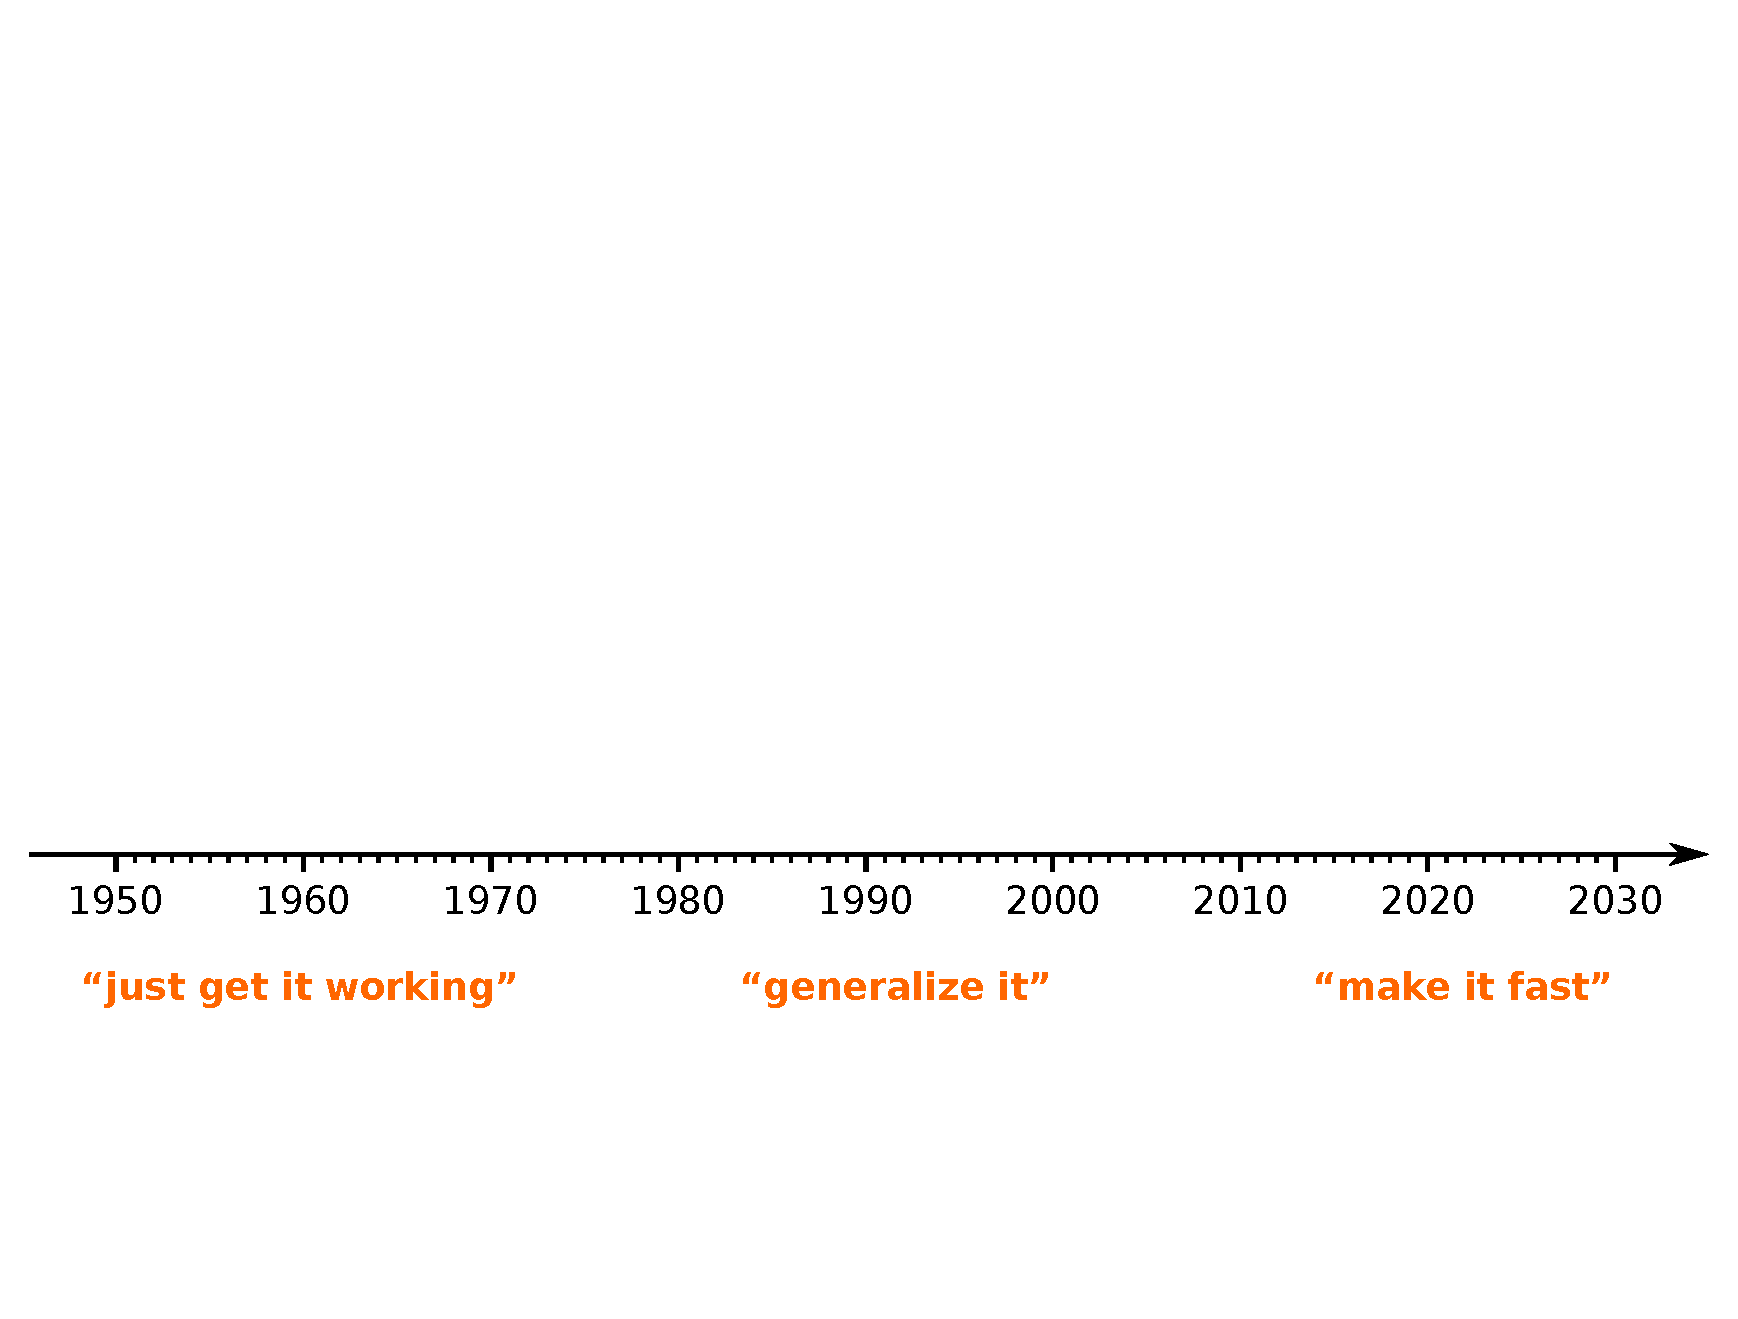
\includegraphics[width=0.88\linewidth]{img/big-oversimplfied-history-8.pdf}}\only<2>{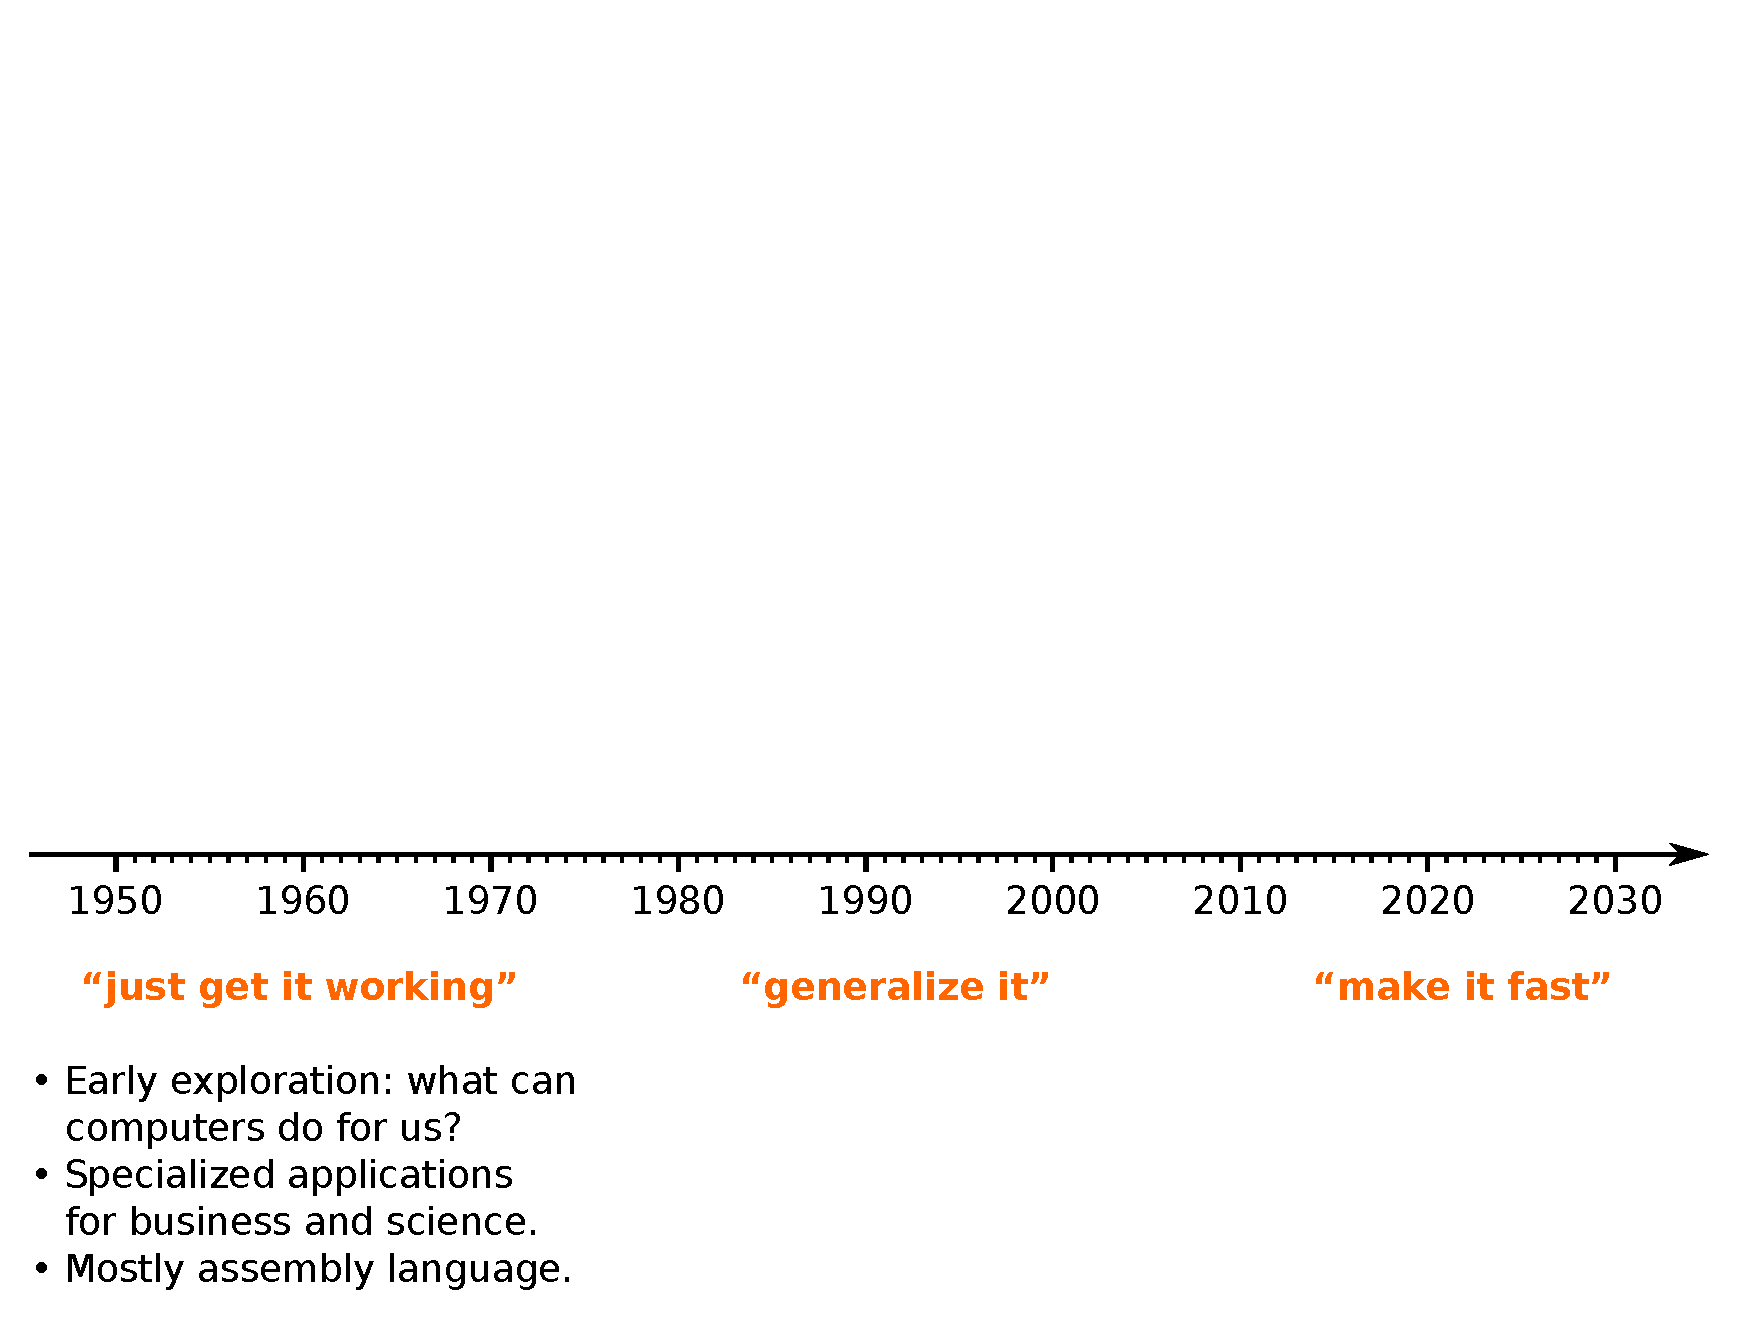
\includegraphics[width=0.88\linewidth]{img/big-oversimplfied-history-7.pdf}}\only<3>{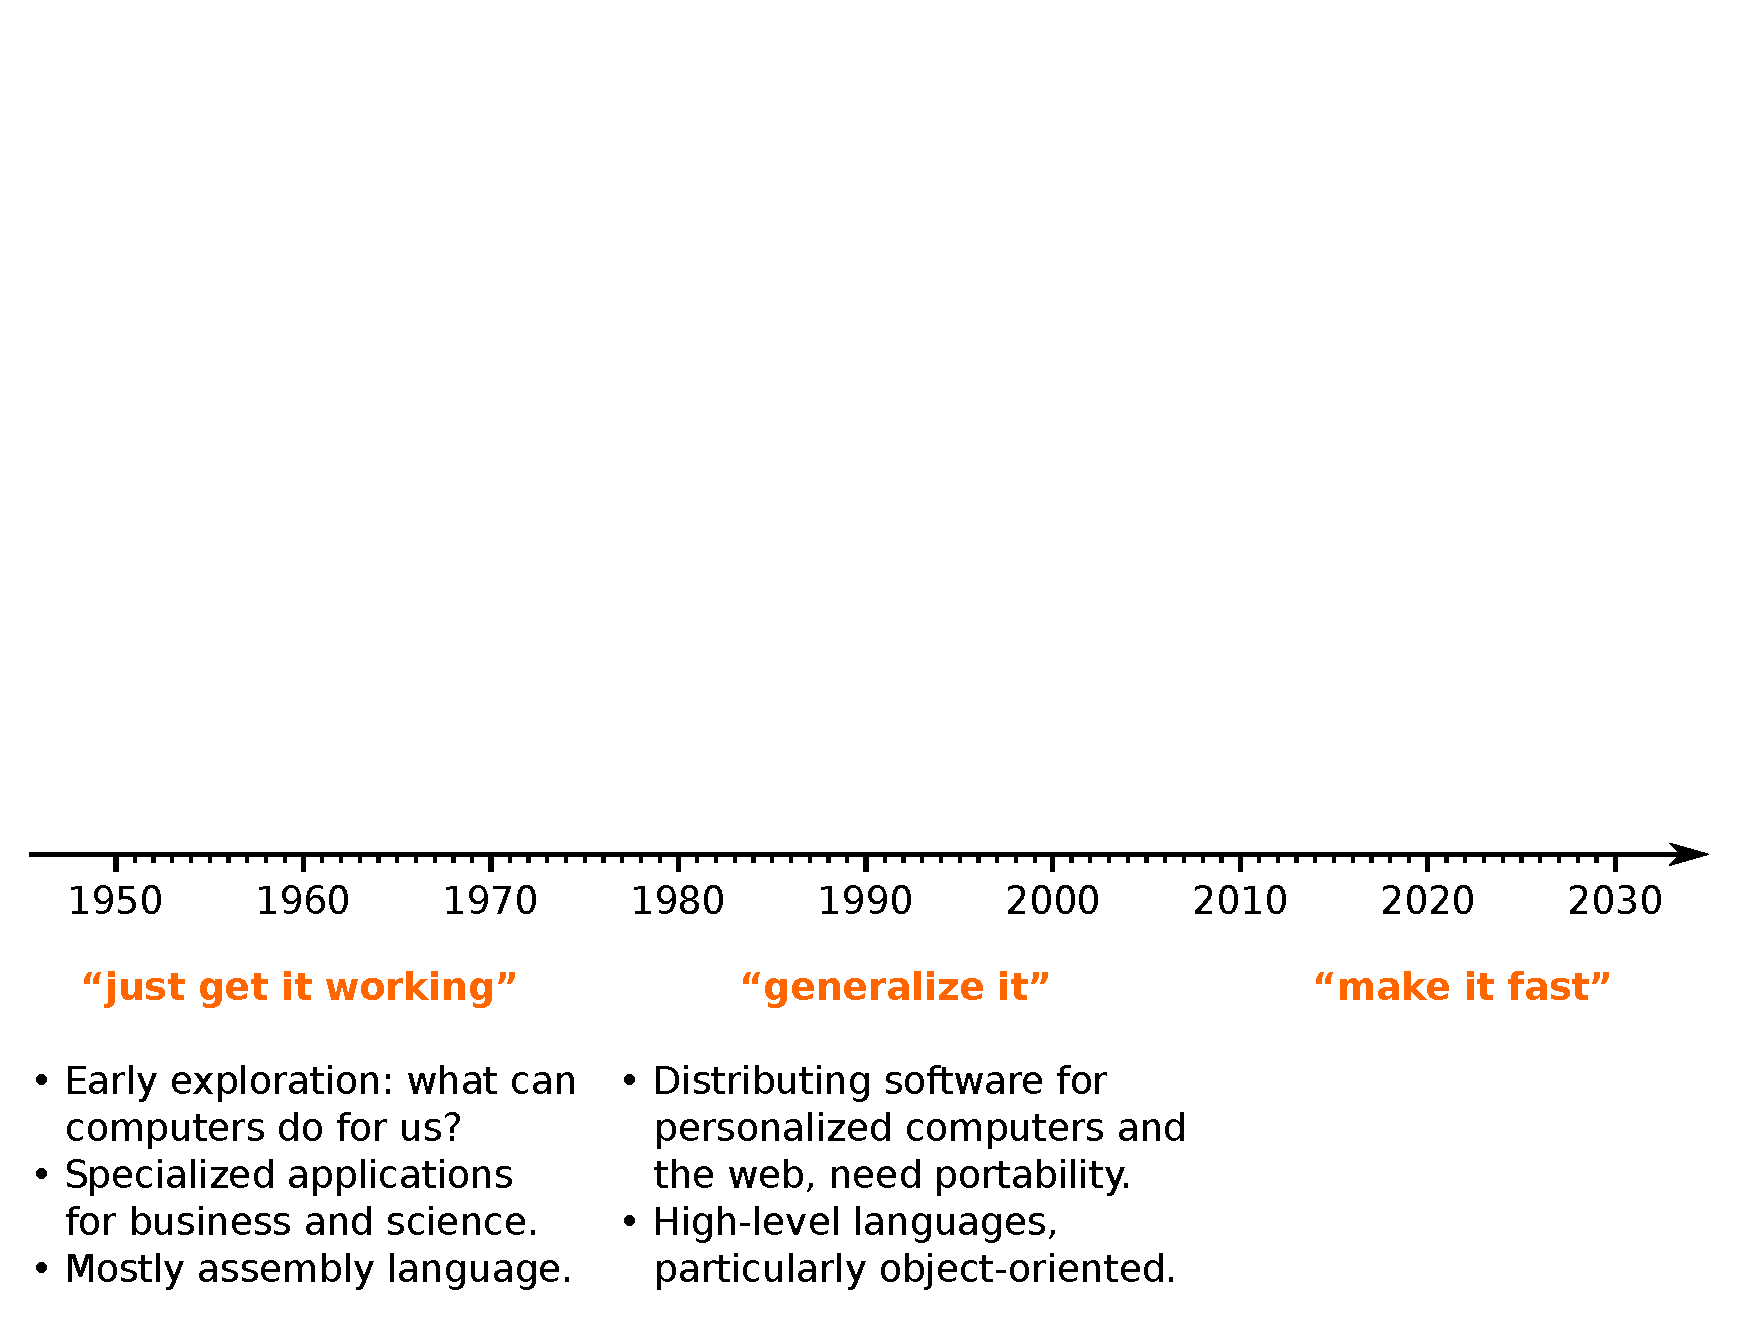
\includegraphics[width=0.88\linewidth]{img/big-oversimplfied-history-6.pdf}}\only<4>{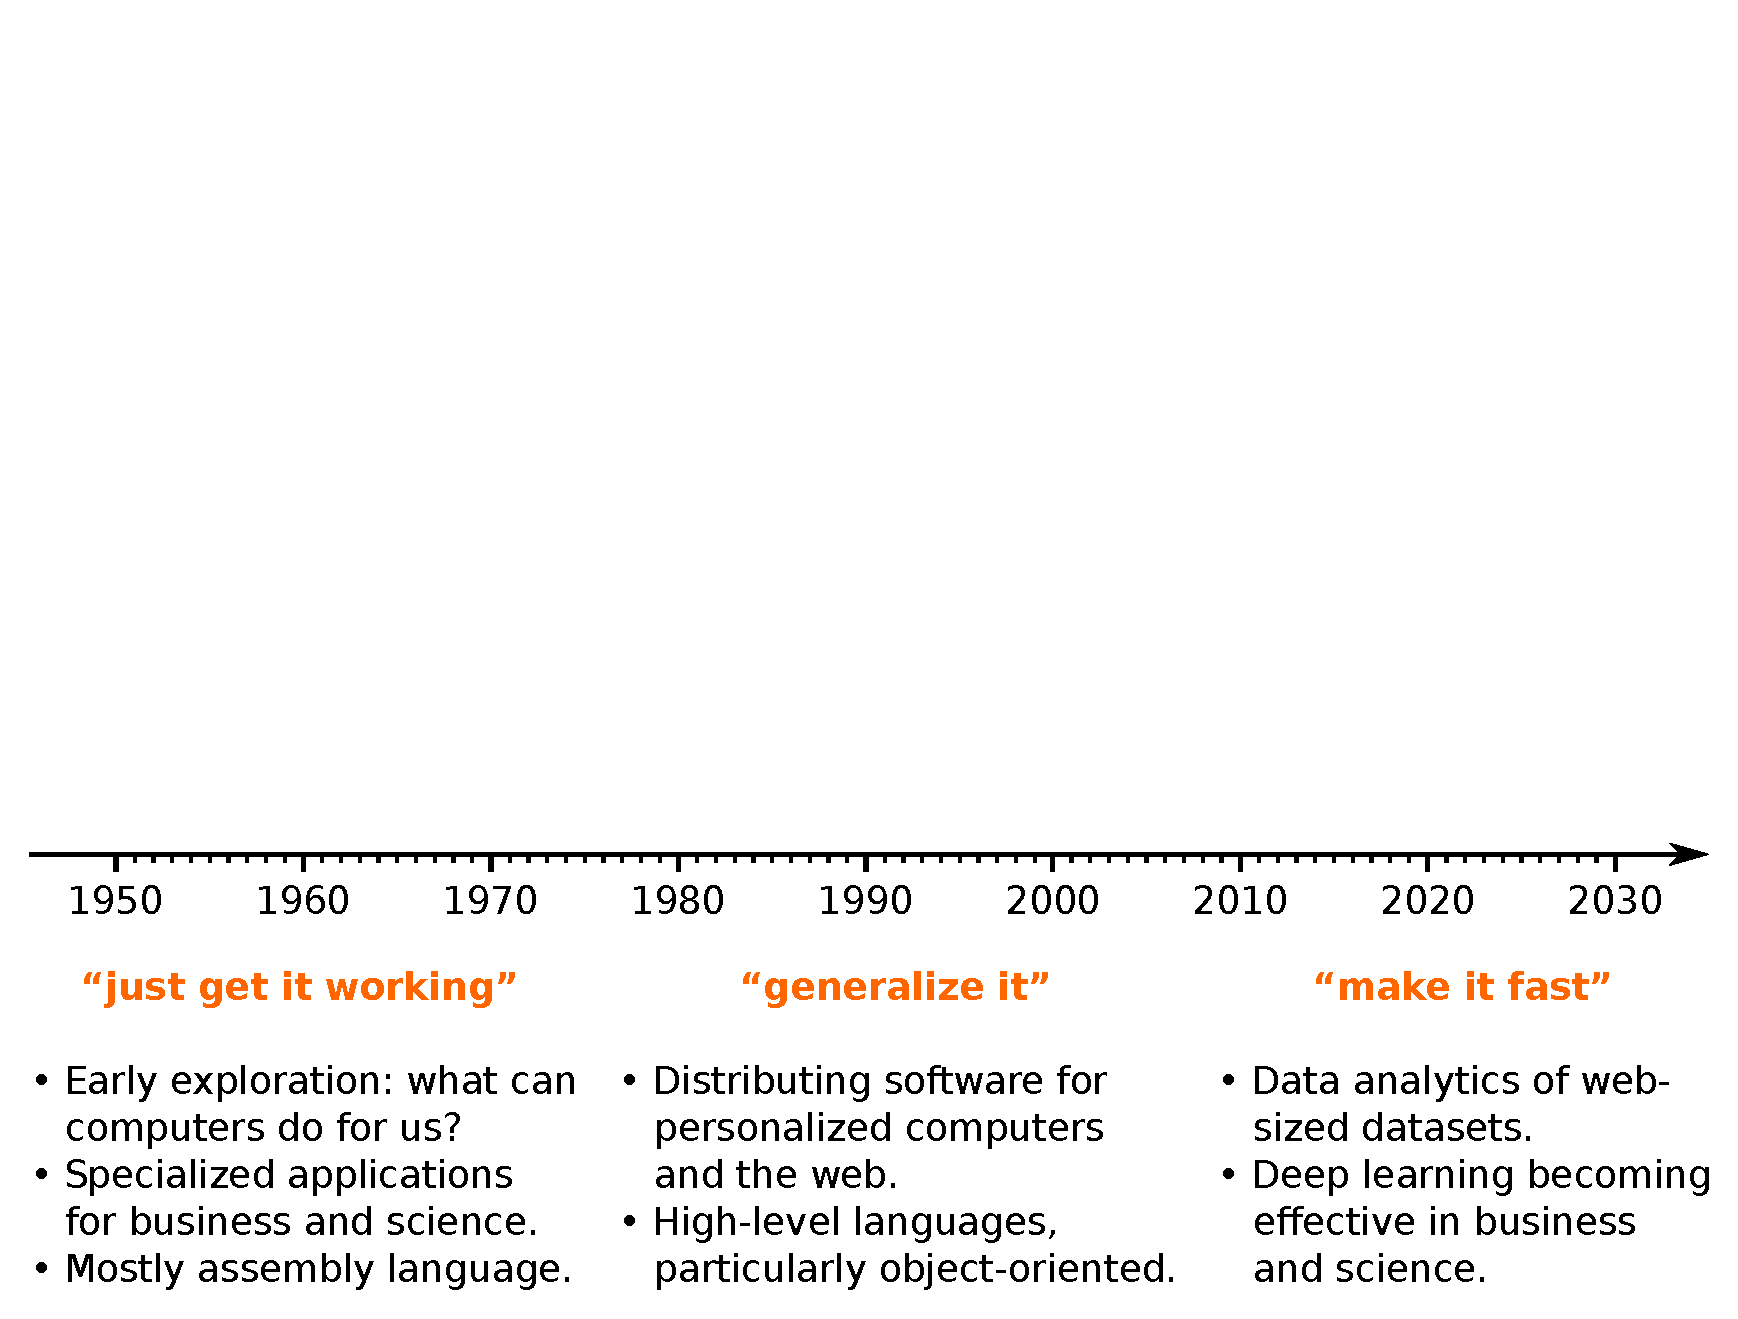
\includegraphics[width=0.88\linewidth]{img/big-oversimplfied-history-5.pdf}}\only<5>{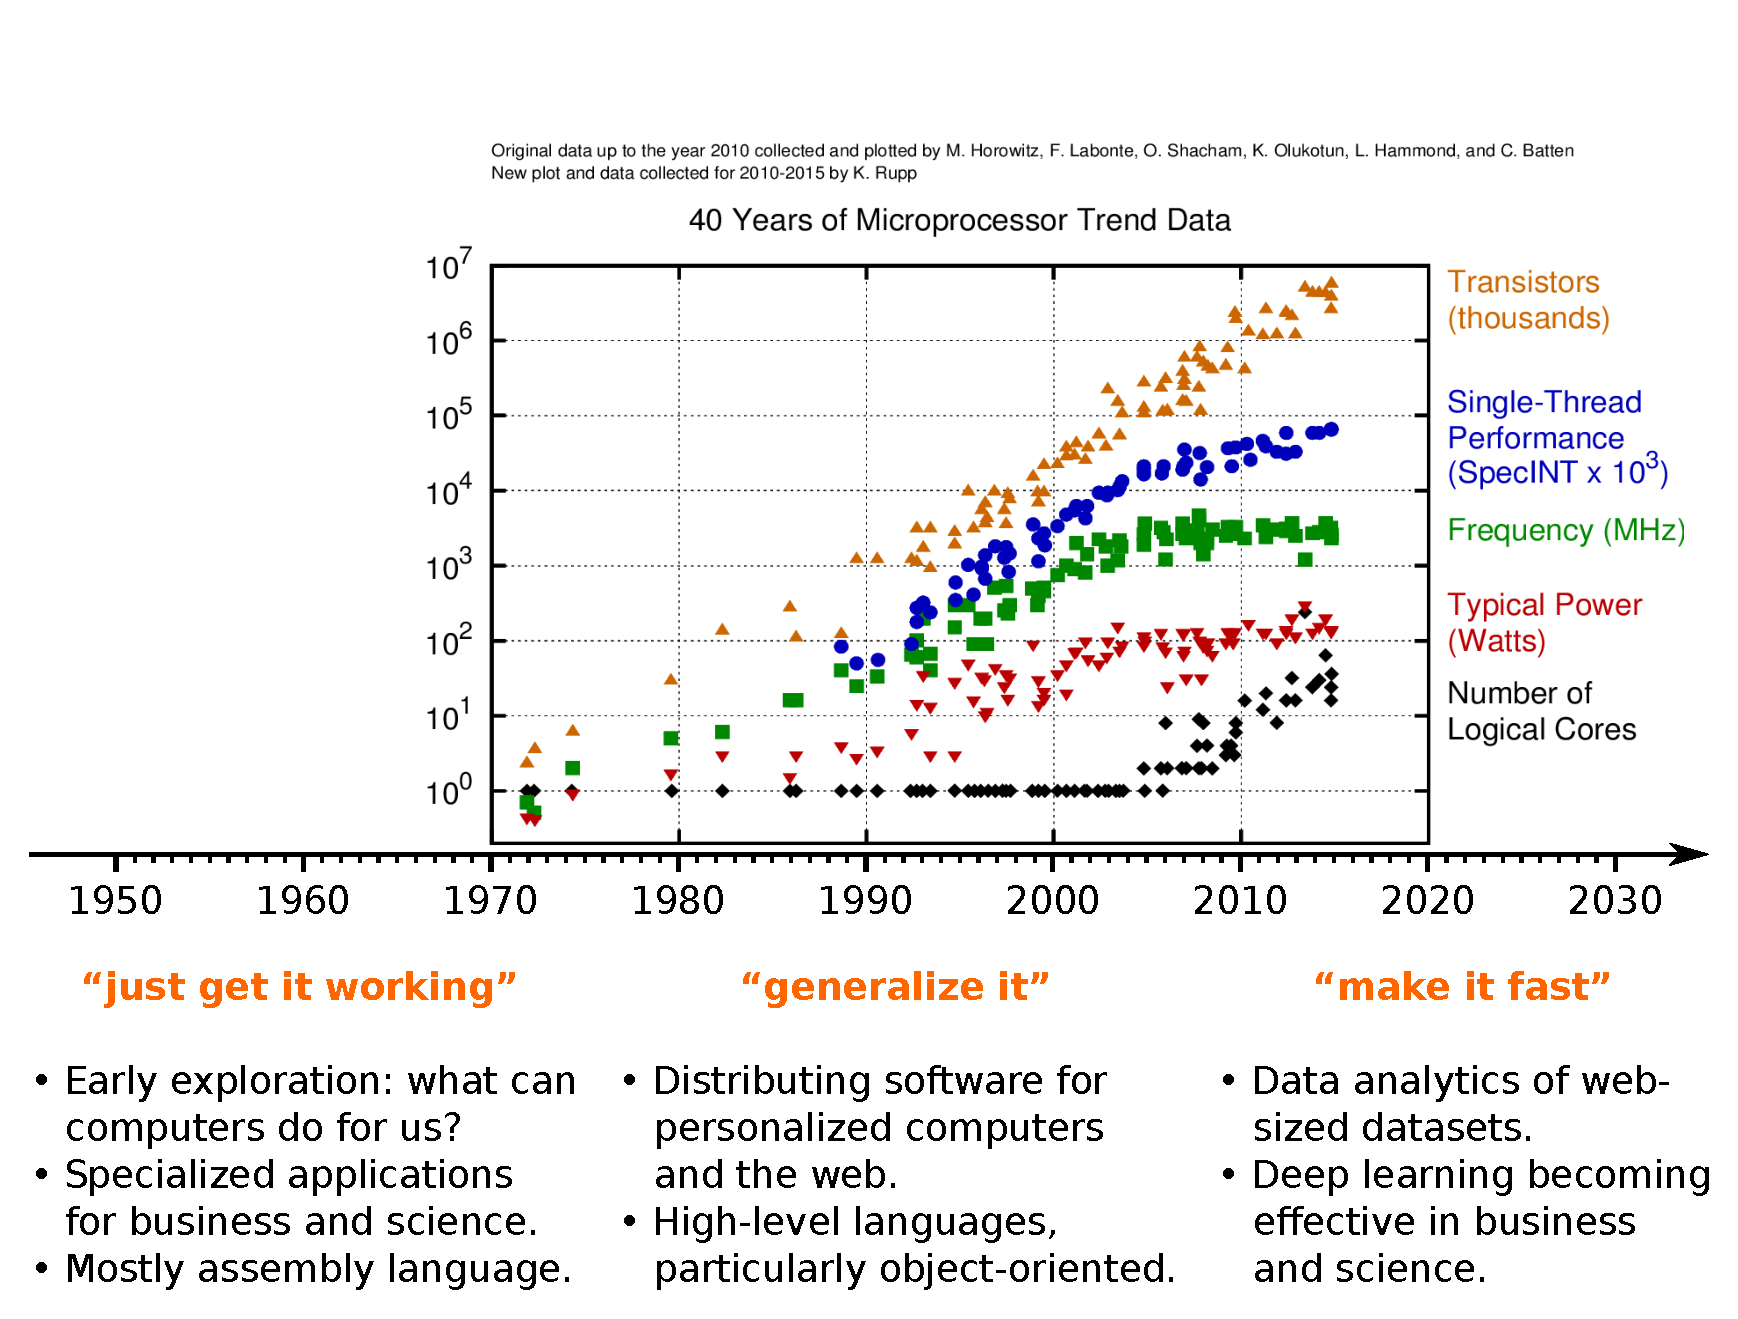
\includegraphics[width=0.88\linewidth]{img/big-oversimplfied-history-4.pdf}}\only<6>{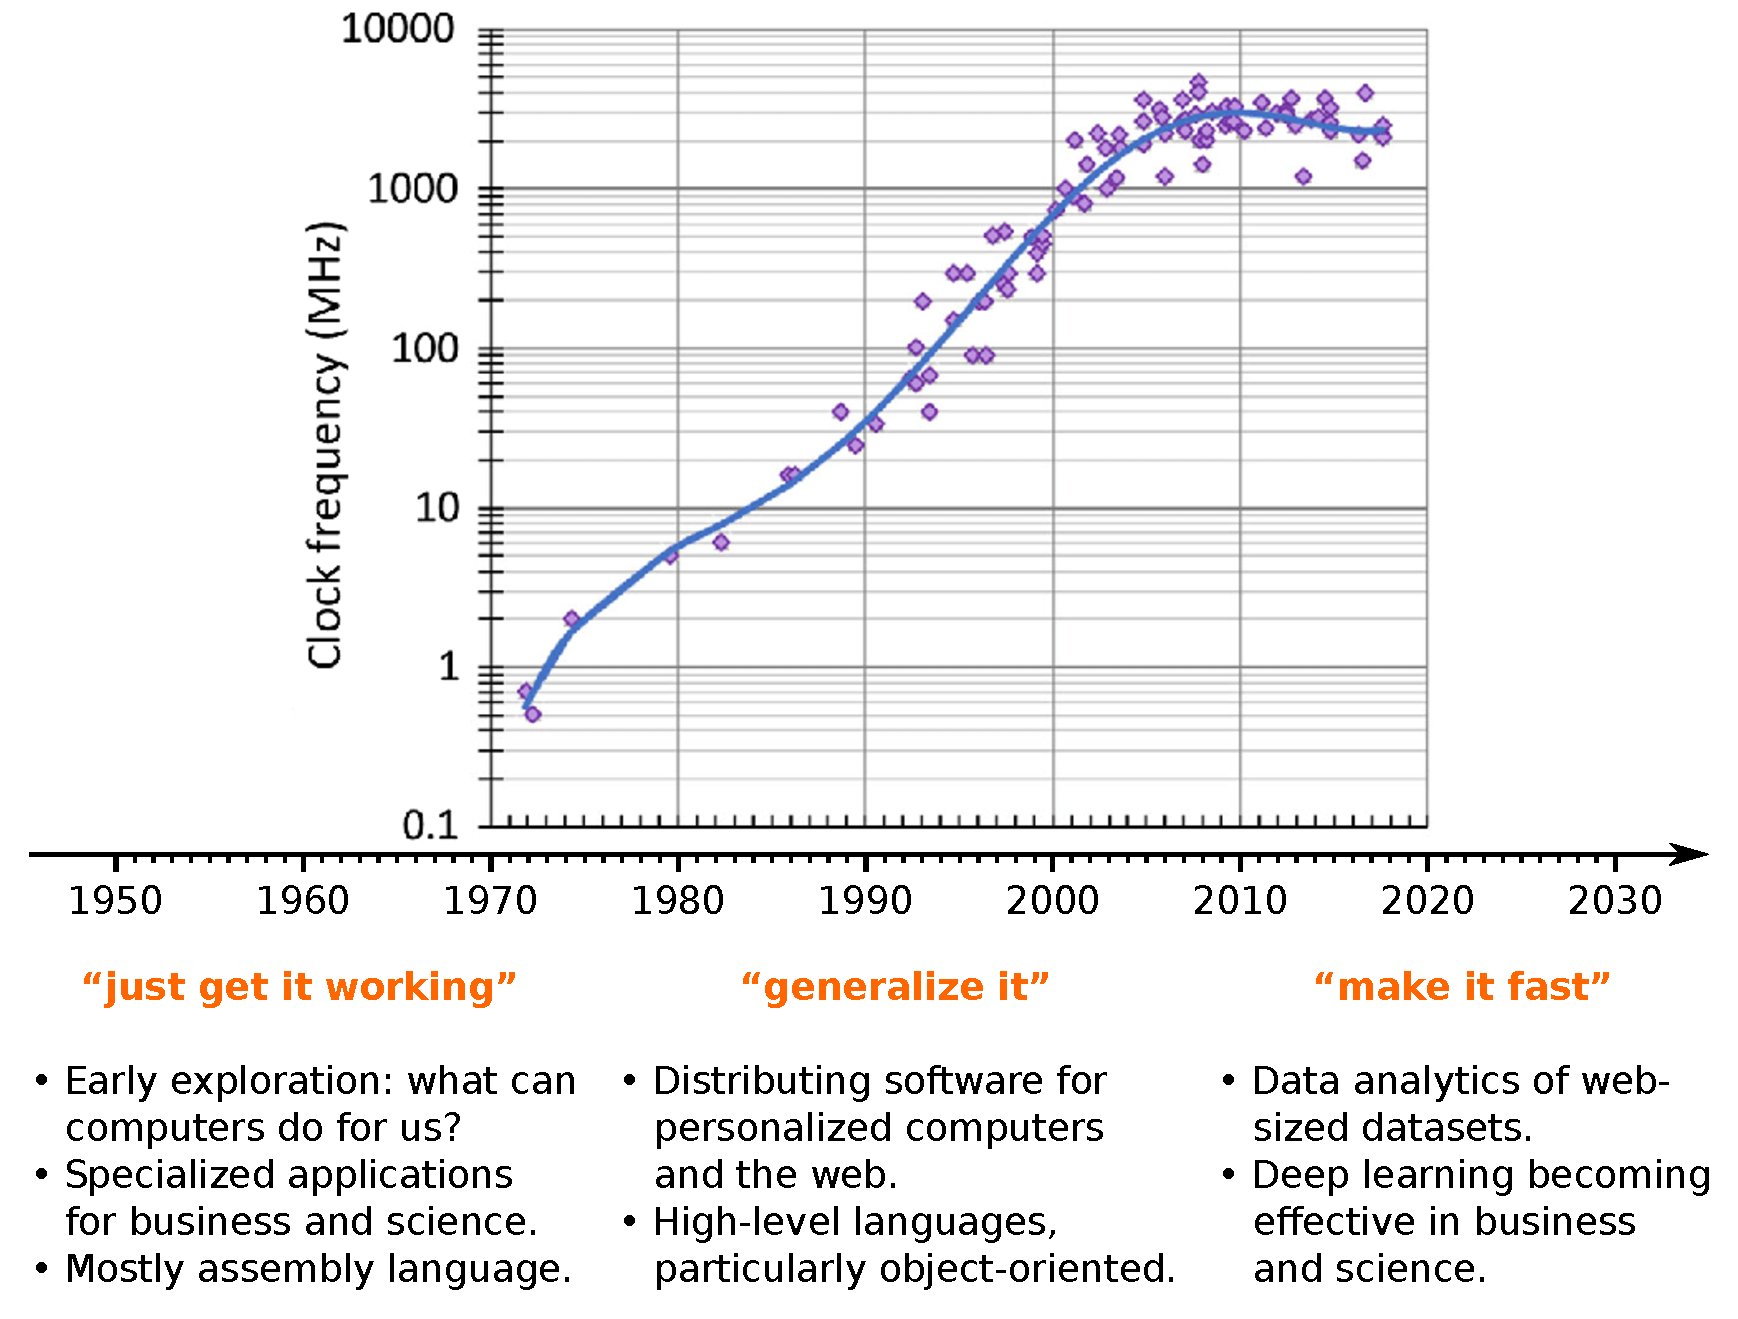
\includegraphics[width=0.88\linewidth]{img/big-oversimplfied-history-3.pdf}}\only<7>{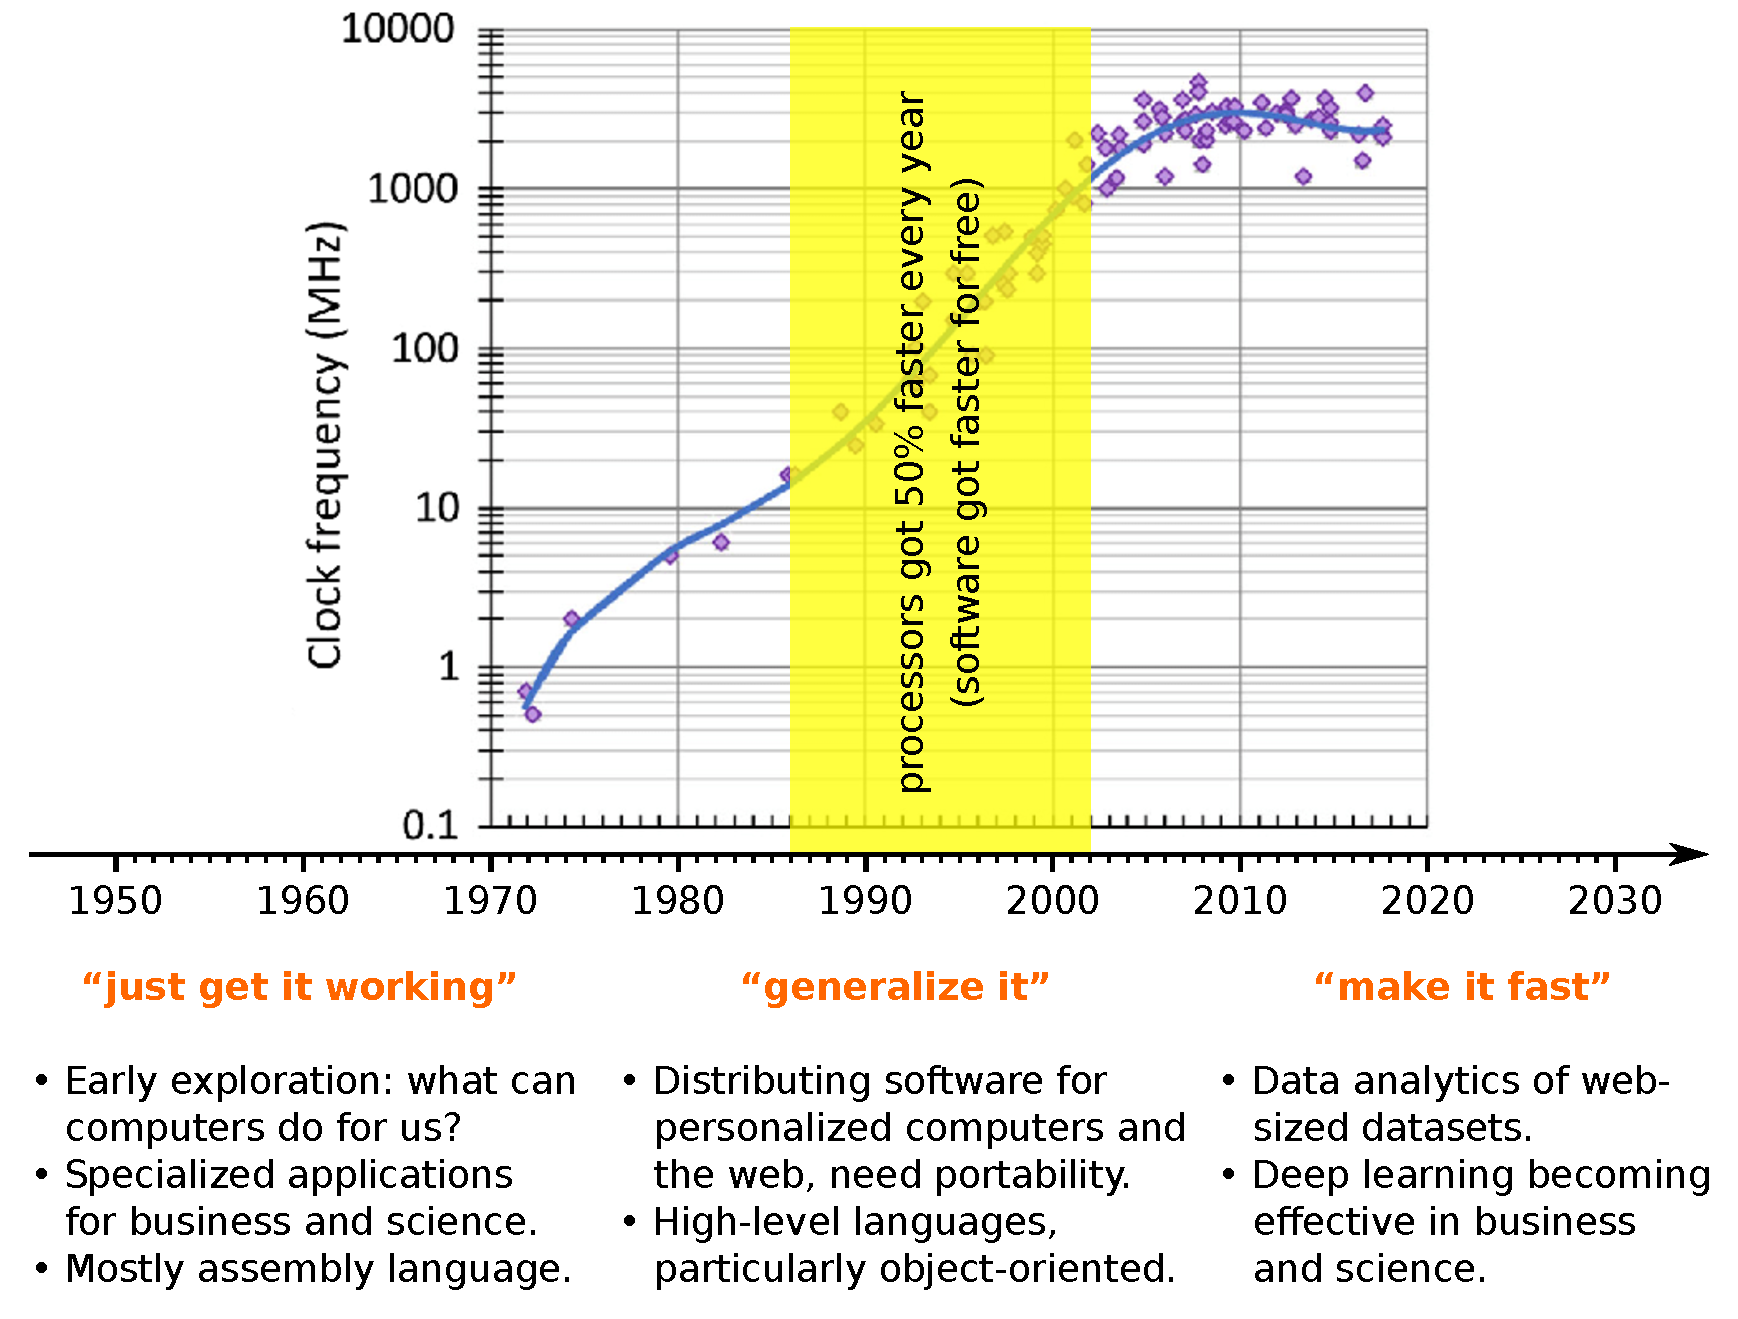
\includegraphics[width=0.88\linewidth]{img/big-oversimplfied-history-2.pdf}}\only<8>{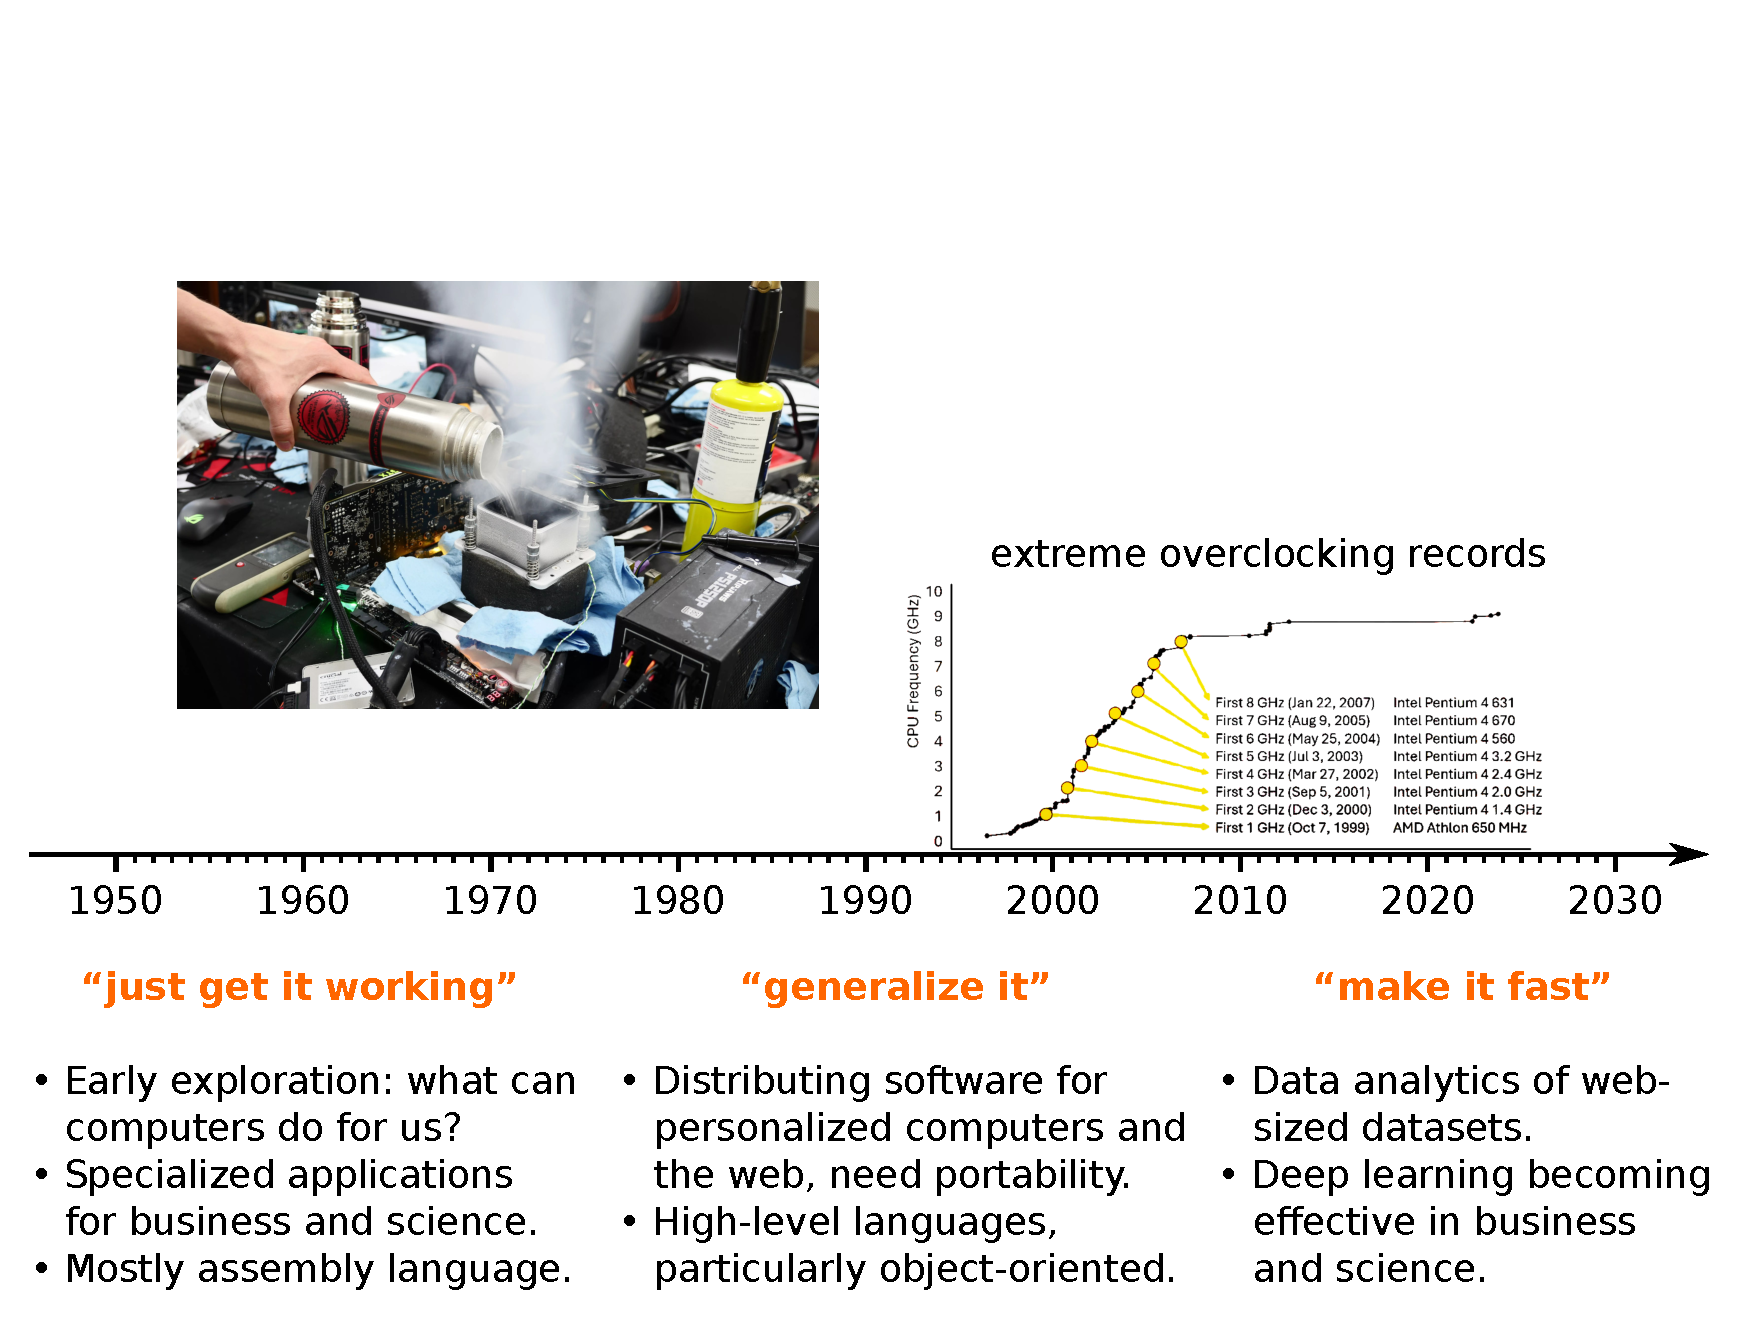
\includegraphics[width=0.88\linewidth]{img/big-oversimplfied-history-1.pdf}}
\end{center}
\end{frame}


\end{document}
